\chapter{Near Elliptical Billiard}

\section{Billiard Mapping}

We define the boundary of a near elliptical billiard to be
\[
    a x^2 + b y^2 + \varepsilon x^4 = 1.
\]
We begin by discussing the details needed for the construction of the billiard map that describes the dynamics of this problem. The radius of the boundary expressed in polar coordinates is given by
\begin{align}
          1 &=  R^2(a\cos^2\theta + b\sin^2\theta)  + R^4(\varepsilon\cos^4\theta) \\
          0 &= -1 + x(a\cos^2\theta + b\sin^2\theta)  + x^2(\varepsilon\cos^4\theta) \hspace{10mm} (x = R^2) \\
            R^2 = x &= \frac{-(a\cos^2\theta + b\sin^2\theta) \pm \sqrt{(a\cos^2\theta + b\sin^2\theta)^2 + 4(\varepsilon\cos^4\theta)}}{2(\varepsilon\cos^4\theta)} \\
R(\theta,a,b,\varepsilon) &= \sqrt{\frac{-(a\cos^2\theta + b\sin^2\theta) \pm \sqrt{(a\cos^2\theta + b\sin^2\theta)^2 + 4(\varepsilon\cos^4\theta)}}{2(\varepsilon\cos^4\theta)} } .
\end{align}
Given an initial position and direction $(\theta_n,\alpha_n)$, the angle between the vector tangent to the curve and the vector perpendicular to the reflected trajectory is given as
\begin{equation}
    \phi_n = \arctan\Big(\frac{Y'(\theta_n)}{X'(\theta_n)}\Big)
\end{equation}
where 
\begin{equation}
    X(\theta_n) = R(\theta_n)\cos(\theta_n)
\end{equation}
\begin{equation}
    Y(\theta_n) = R(\theta_n)\sin(\theta_n)
\end{equation}
and their derivatives are
\begin{equation}
    X'(\theta_n) = R'(\theta_n)\cos(\theta_n) - R(\theta_n)\sin(\theta_n) 
\end{equation}
and
\begin{equation}
    Y'(\theta_n) = R'(\theta_n)\sin(\theta_n) + R(\theta_n)\cos(\theta_n).
\end{equation}
To obtain the new position $\theta_{n+1}$ we must solve the equation
\begin{equation}
    Y(\theta_{n+1}) - Y(\theta_n) = \tan(\alpha_n + \phi_n)(X(\theta_{n+1}) - X(\theta_n))
\end{equation}
As seen in figure \ref{billiardmap} the next trajectory angle $\alpha_{n+1}$ is given by
\begin{equation}
    \alpha_{n+1} = \phi_{n+1} - (\alpha_n + \phi_n)
\end{equation}
Thus the billiard mapping is defined as
\begin{equation}
    \begin{cases} 
      F(\theta_{n+1}) = 0 = Y(\theta_{n+1}) - Y(\theta_n) - \tan(\alpha_n + \phi_n)(X(\theta_{n+1}) - X(\theta_n)) \\
      \alpha_{n+1} = \phi_{n+1} - (\alpha_n + \phi_n)
   \end{cases}
   \label{bmap}
\end{equation}

\section{Numerical Results}
Let us now discuss some of our results. Figures \ref{nearellipse1}, \ref{nearellipse2}, and \ref{nearellipse3} illustrate the destruction of both the confocal caustic and invariant curve in the phase space as we increase the parameter $\varepsilon$. As shown in Figures \ref{nearellipse4} and \ref{nearellipse5} we can see a complex hierarchy of behaviours in the phase space along with the formation of a large chaotic sea as we increase $\varepsilon$. 
\begin{figure}[h]
    \centering
    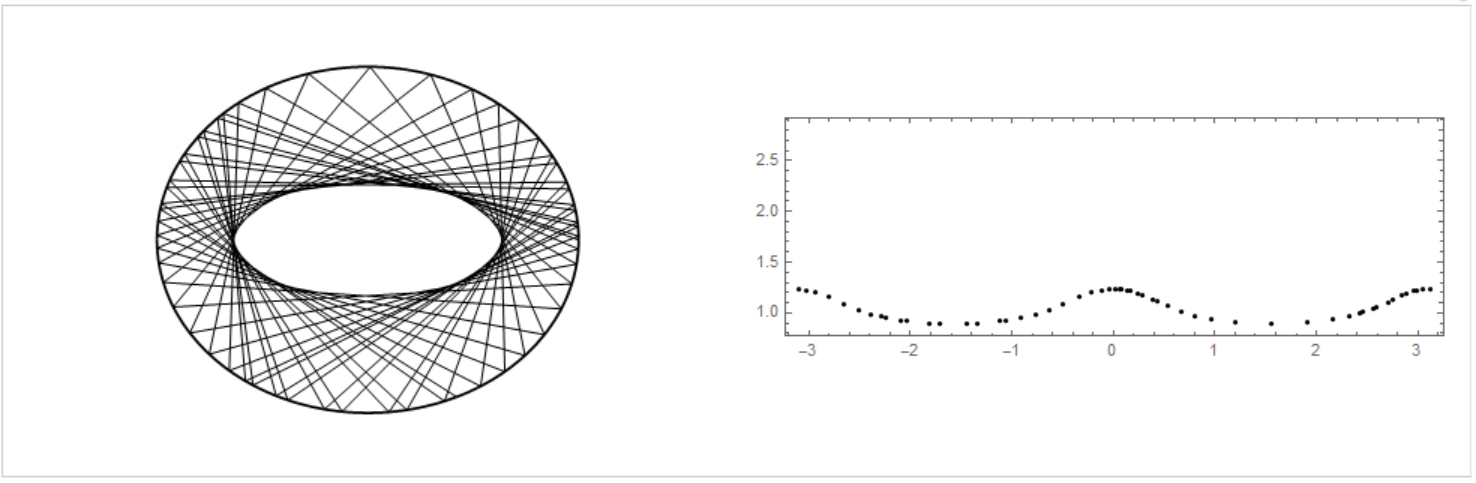
\includegraphics[width = 0.9\textwidth]{NearellipsePhaseSpace2}
    \caption{Near elliptical Billiard $a=1, b=1.5, \varepsilon = .01$ with Phase Space Diagram}
    \label{nearellipse1}
\end{figure}
\begin{figure}[h]
    \centering
    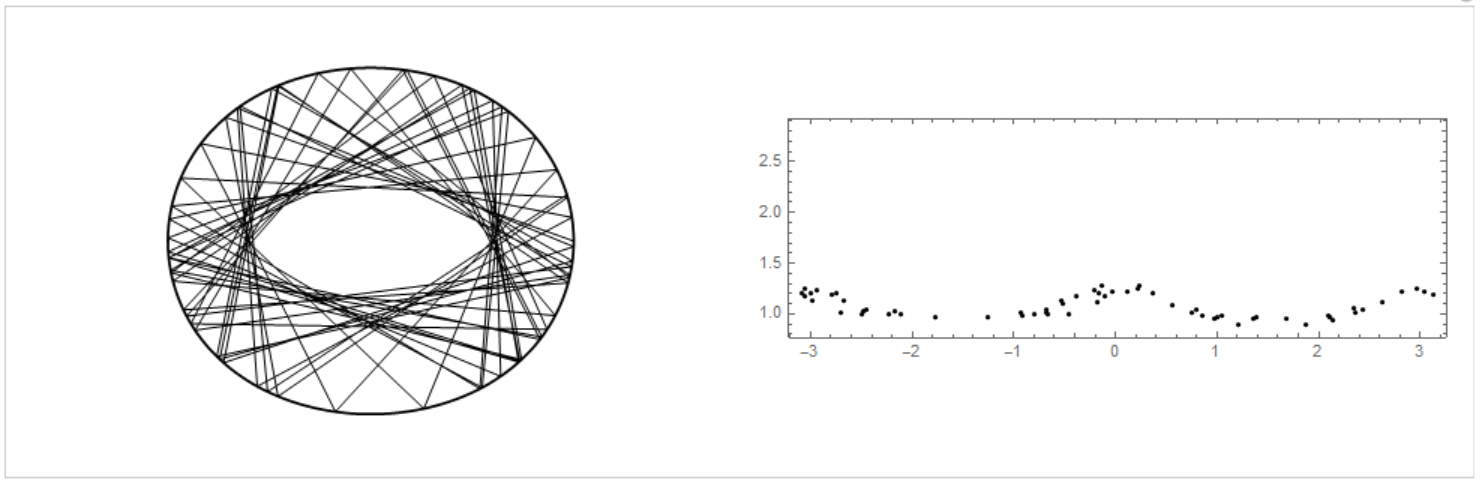
\includegraphics[width = 0.8\textwidth]{NearellipsePhaseSpace3}
    \caption{Near elliptical Billiard $a=1, b=1.5, \varepsilon = .1$ with Phase Space Diagram}
    \label{nearellipse2}
\end{figure}
\begin{figure}[h]
    \centering
    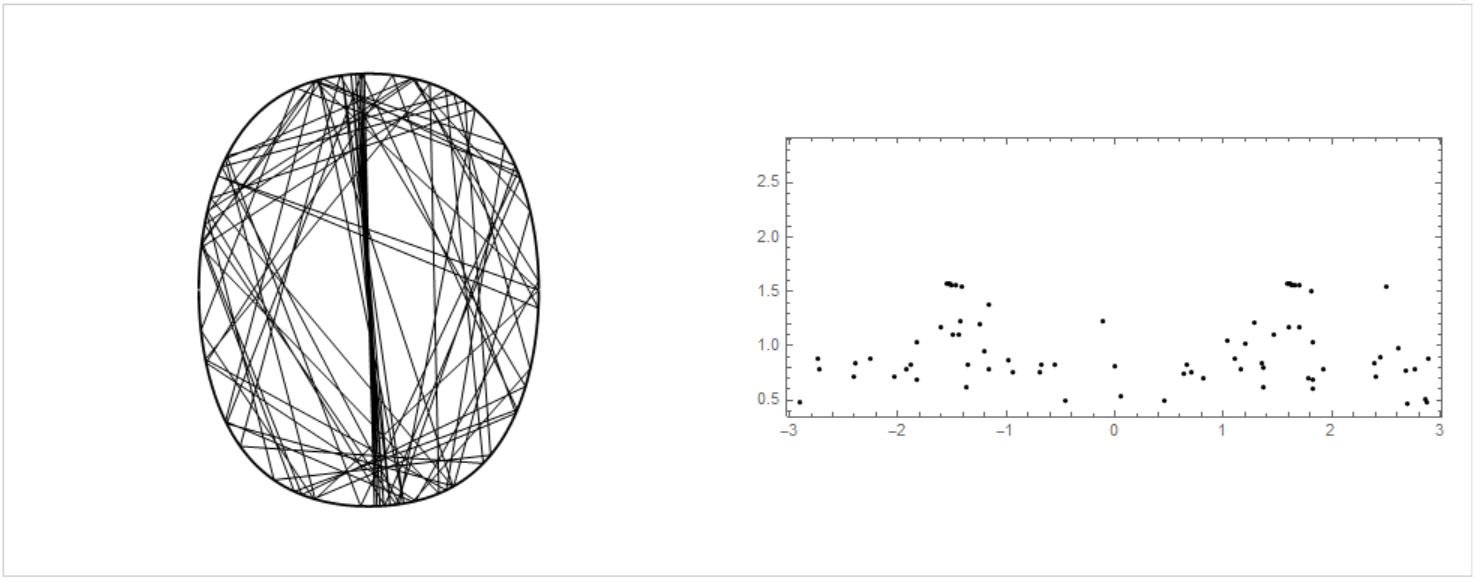
\includegraphics[width = 0.8\textwidth]{NearellipsePhaseSpace}
    \caption{Near elliptical Billiard $a=b=\varepsilon = 1$ with Phase Space Diagram}
    \label{nearellipse3}
\end{figure}

\begin{figure}[h]
    \centering
    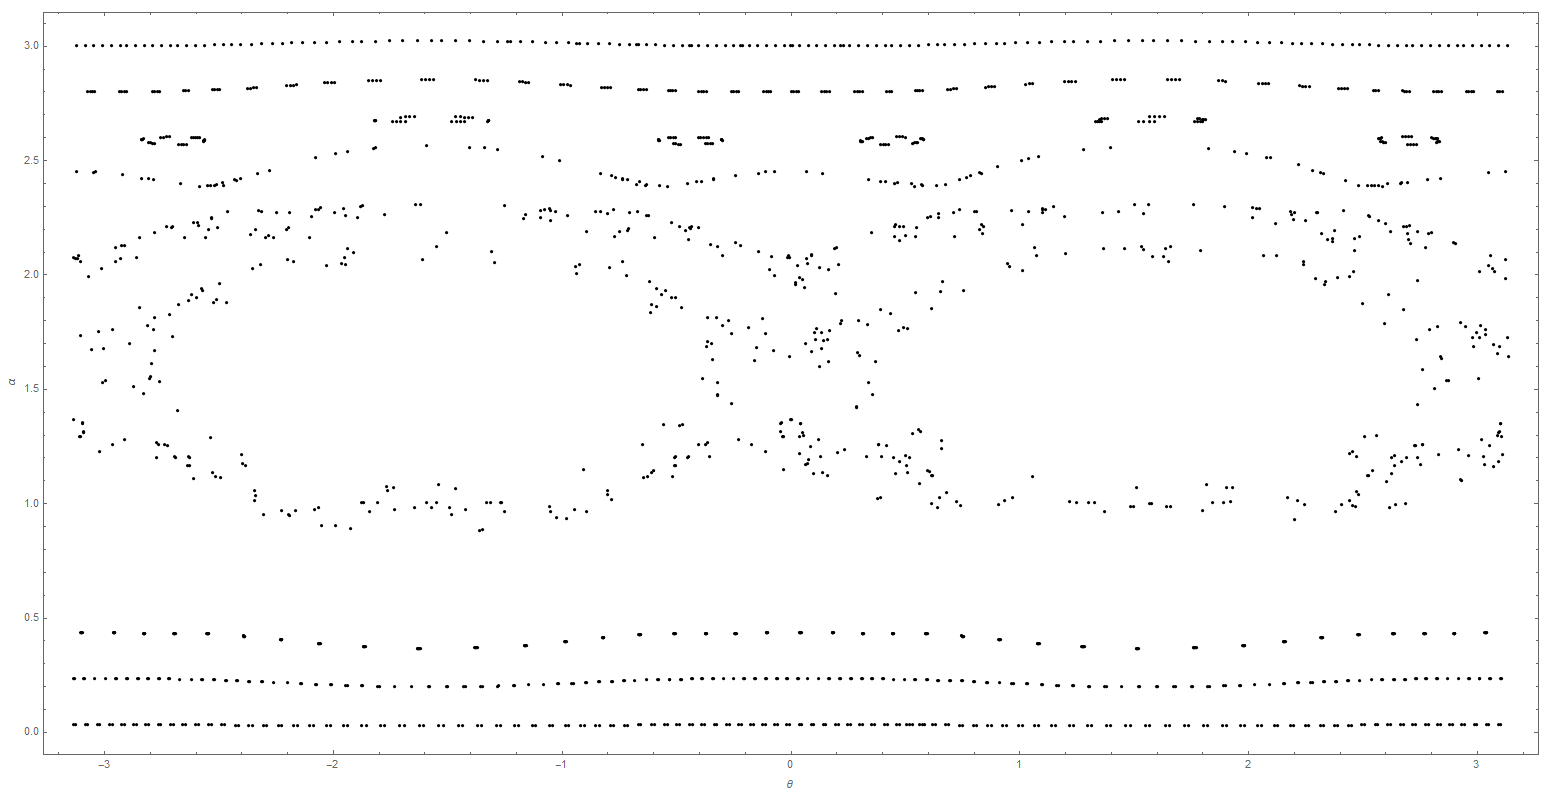
\includegraphics[width = 0.9\textwidth]{NearellipsePhaseSpace4}
    \caption{Near elliptical Billiard $a=1, b=1.5, \varepsilon = .1$ with Phase Space Diagram}
    \label{nearellipse4}
\end{figure}
\begin{figure}[h]
    \centering
    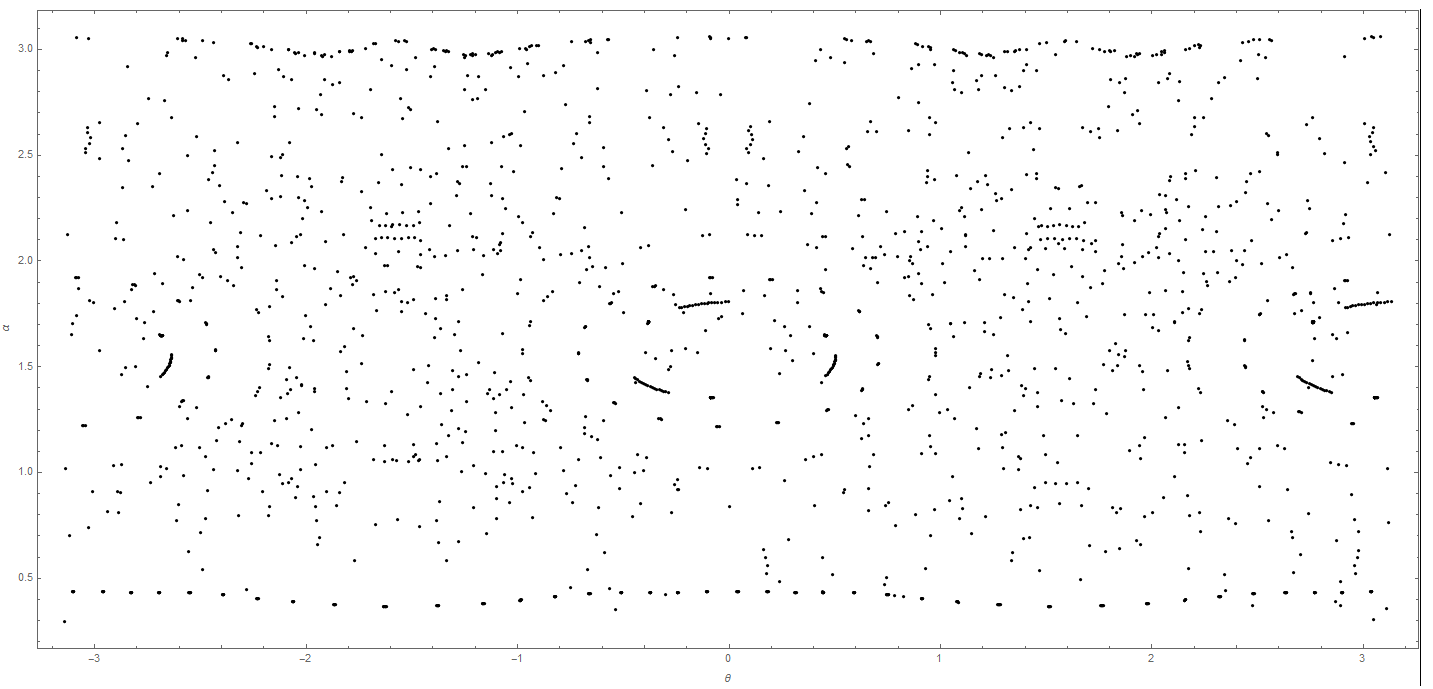
\includegraphics[width = 0.9\textwidth]{NearellipsePhaseSpace5}
    \caption{Near elliptical Billiard $a=1, b=1.5, \varepsilon = 10$ with Phase Space Diagram}
    \label{nearellipse5}
\end{figure}
Qualitatively, it is simple to see from the phase space diagrams that as we perturb an ellipse by increasing $\varepsilon$, the billiard no longer is integrable. To obtain a more quantitative sense of this chaotic motion we examine the Lyapunov exponent.
\begin{definition}
As discussed in \cite{Oliveira2010}, the \textbf{Lyapunov exponent} is defined as
\[
    \lambda_j = \lim_{n \rightarrow \infty} n^{-1} \log |\Lambda_j| \hspace{10mm} j = 1,2
\]
where $\Lambda_j$ are the eigenvalues of $M = \prod_{i = 1}^n J_i(\theta_i, \alpha_i)$ and $J_i$ is the Jacobian matrix evaluated over the orbit $(\theta_i, \alpha_i)$.
\end{definition}
It is well known that the Lyapunov exponent serves as a practical tool for studying the behavior of a dynamical system, and consequently whether the given system is chaotic. If the Lyapunov exponent converges to a positive value after significantly large $n$ we say that our system is chaotic. 
\newpage
Since our billiard mapping \ref{bmap} is not well defined to compute the product of Jacobians, we discuss a method to compute the Lyapunov exponents numerically. 
\begin{enumerate}
    \item Starting with initial conditions $\theta_{u0}$ and $\alpha_{u0}$ (call orbit $u$), choose a nearby point $(\theta_{v0}, \alpha_{v0})$ (call orbit $v$) that is within distance $d_0$.
    \item
    Iterate both orbits once and calculate the new distance $d_1$.
    \item
    Evaluate $\ln(d_1/d_0)$.
    \item
    Readjust the point along orbit $v$ so that its distance from the new point on orbit $u$ is $d_0$ and in the same direction as $d_1$. i.e.
    \[
        \theta_{v0} = \theta_{u1} + d_0(\theta_{v1} - \theta_{u1}) / d_1
    \] and
    \[
        \alpha_{v0} = \alpha_{u1} + d_0(\alpha_{v1} - \alpha_{u1}) / d_1
    \]
    \item Repeat steps 2 - 4 $n$ times and calculate a running average of step 3. 
\end{enumerate}
This process is illustrated in Figure \ref{dia}. 

\begin{figure}
    \centering
    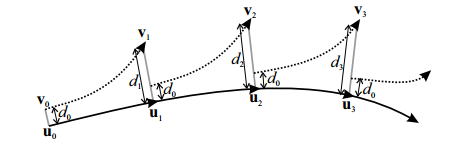
\includegraphics{diagram}
    \caption{Diagram of how to compute the Lyapunov Exponent numerically}
    \label{dia}
\end{figure}
Due to the precision of floating point numbers in Mathematica, we choose $d_0 = 10^{-8}$. To illustrate that our near elliptical billiard has a chaotic component in the phase space, we show in Figures \ref{lyap1} and \ref{lyap2} the behavior of the positive Lyapunov exponent as a function of the number of collisions $n$ for various initial conditions chosen in the chaotic sea. Each initial condition was iterated up to $500$ times. 
\begin{figure}
    \centering
    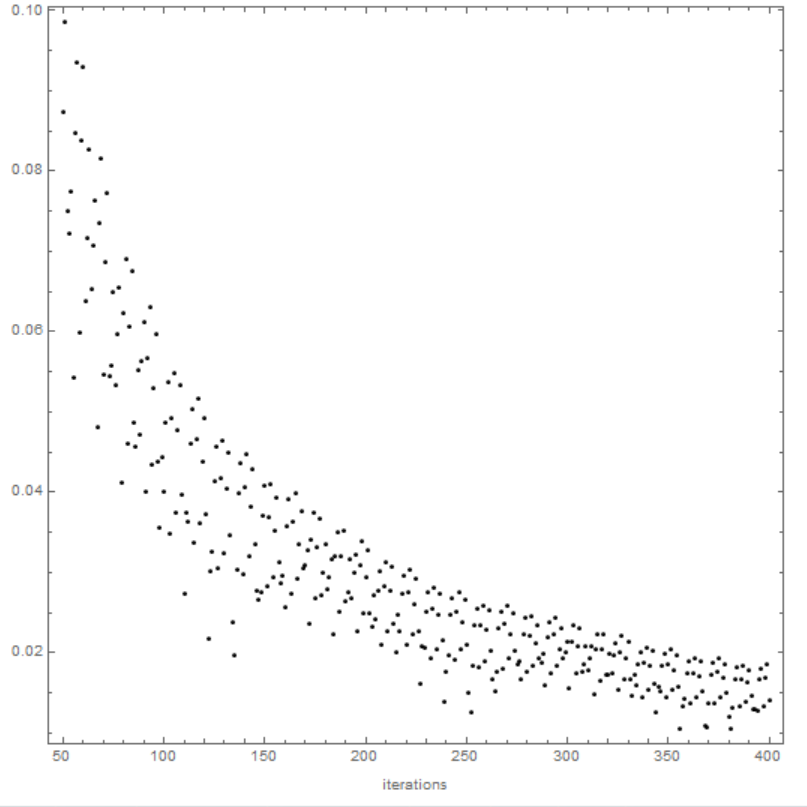
\includegraphics{lyap1}
    \caption{Behavior of the Lyapunov Exponent for $a = 1$, $b = 1.4$, and $\varepsilon$ = 1.5}
    \label{lyap1}
\end{figure}
\begin{figure}
    \centering
    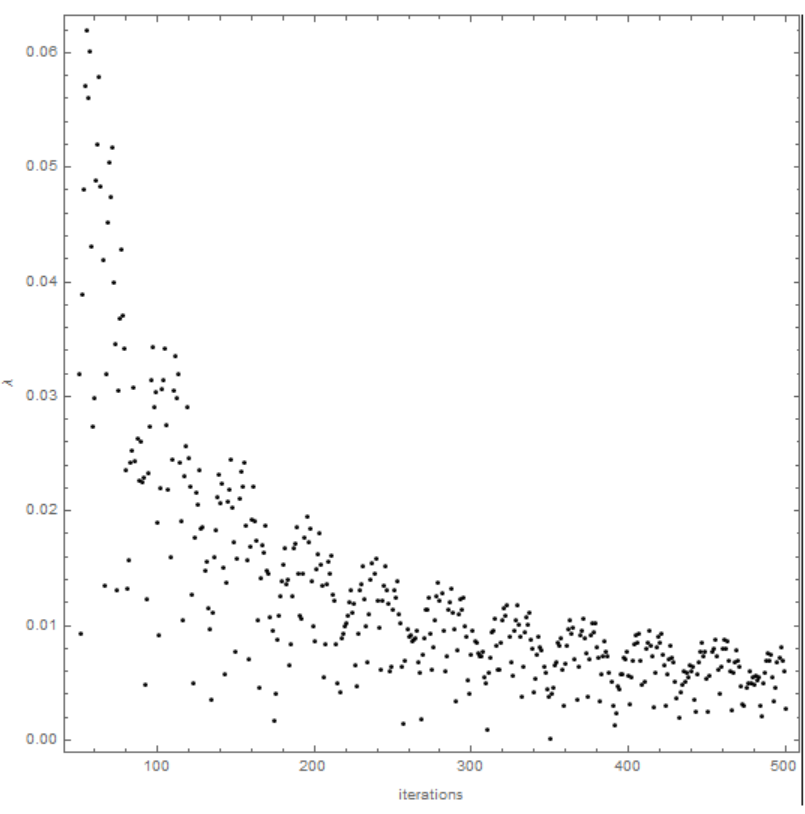
\includegraphics{lyap2}
    \caption{Behavior of the Lyapunov Exponent for $a = 1$, $b = 1.4$, and $\varepsilon$ = 0.1}
    \label{lyap2}
\end{figure}

In future work, many more iterations are needed to provide a proper convergence plot of the positive Lyapunov exponent. However, it is still clear to see from the plots that it will eventually converge to a positive value. As such we can conclude that the regions of our phase space for near elliptical billiards are chaoitic and that the system is no longer integrable due to the destruction of the invariant spanning curves in the phase space. 